\documentclass[a4paper]{article}
\usepackage[utf8]{inputenc}
\usepackage{graphicx}
\usepackage{twocolpceurws}
\usepackage{xcolor}
\usepackage{url}

\def\infinity{\rotatebox{90}{8}}


\title{Damegender: Towards an International and Free Dataset about Name, Gender and Frequency}

\author{
David Arroyo Menéndez \\ Grupo de Sistemas y Comunicaciones (GSyC) \\ Universidad Rey Juan Carlos, Madrid, Spain \\ \{d.arroyome@alumnos\}.urjc.es
}
%% Alexander Serebrenik
%% Jesus González-Barahona, Gregorio Robles

\newif\ifdraft
\drafttrue
%\draftfalse
\newcommand{\nb}[2]{
	{
		{\color{black}{
				\small\fbox{\bfseries\sffamily\scriptsize#1}
				{\sffamily\small$\triangleright~${\it\sffamily\small #2}$~\triangleleft$}
	}}}
}


\ifdraft
\newcommand\davidam[1]{\nb{David}{\color{olive}#1}}
\newcommand\grex[1]{\nb{Gregorio}{\color{red}#1}}
\newcommand\jgb[1]{\nb{Jesús{\color{blue}#1}}}
\newcommand\fixme[1]{{\textcolor{red}{[FIXME] #1}}}
\newcommand\cn{{\color{violet}[citation required]}}

\else
\usepackage[disable]{todonotes}
\newcommand\gema[1]{}
\newcommand\grex[1]{}
\newcommand\mei[1]{}
\newcommand\fixme[1]{}
\newcommand\cn{}


\fi
\let\labelindent\relax
\usepackage[inline]{enumitem}





\institution{}


\begin{document}

\maketitle

\begin{abstract}
  %% Introduction

  Equality of gender is the 5th objective of sustanaible development
  in United
  Nations\footnote{https://www.un.org/sustainabledevelopment/gender-equality/}.

  This equality can be reached working on to measure and to analyze
  data and to apply politics from the results. On many gender studies,
  we need to count males and females deciding gender from names, for
  instance, research papers, job positions, streets, ... The
  traditional way is to use commercial APIs with propietary data
  without idea about how the data has been built. Another way, is
  taking data from wikipedia or scientific sites.

  %% Methodology

  With Open Data idea, many statistics institutions are providing Open
  Datasets about name, gender and frequency. So, we need a scientific
  discussion about unifying formats, making easy ways to process these
  data and ways towards make standards.

  %% Results
  
  The dataset is covering more than 20 countries in the occidental
  world. Having more names than any open source software in this
  moment. Allowing to measure gender gap to students and academics
  interested on the phenomenon.

  %% Conclusion

  There are a warranty of quality on reproducible research, that's the
  Free Software and the citation about official sources about names,
  gender and frequency provided by statistics institutions making easy
  the peer review and opening doors to the semantic web and the
  attention to diversity.
  
\end{abstract}



\section{Introduction}

Nowadays, many people is using APIs such as Genderapi, Genderize,
Namsor, or NameApi. Another people is using solutions based on
Wikipedia, or free software solutions (NLTK\cite{loper2002nltk}, R
Gender, Gender Detector, Gender
Computer\footnote{https://github.com/tue-mdse/genderComputer}, ...)
with few number of names due to use files of a single country or being
software not maintained in the long time. Wikipedia is not taking into
account the frequency of the names.

However, the gender gap is a problem recognised in United Nations and
the IT market is leading big inequalities in the world in economy and
gender gap. This paper present a real work collecting data with a
scientific perspective to solve the problem.

Another previous work~\cite{karimi2016inferring} about this kind of
tools is discussing about the datasets as a way to improve the
accuracies, comparing tools that is using different public datasets
(SSA, IPUMS, Sexmachine, ...)

We are facing the solution by the practical way augmenting the number
of names using official statistics and taking into account diversity
goals such as non binary gender and cultural minorities.

The remainder of this paper is structured as follows:

In Section~\ref{sec:truehood} we discuss the different ways to find
evidence about names, gender and frequency.

Section~\ref{sec:diversity} introduces the diversity discussion about
minorities.

Section~\ref{sec:semantic} is giving clues about how to approach the
semantic web goals with the previous dicussion presented.

Section~\ref{sec:damegender} reports on values of accuracy and offers
a confusion matrix using a scientific dataset.

Section~\ref{sec:measuring} is about how we use Machine Learning in
\texttt{damegender}.

Section~\ref{sec:conclusions} discusses limitations and further
research, and concludes the paper.

\section{Truehood and Falsehood in names, gender and frequency}
\label{sec:truehood}

The current idea in the field is the data about name, gender and
frequency is ok because there are people who is paying by it, or many
people is downloading a product. This intuition is right generally,
although sometimes the people is paying by a bad product due to a good
marketing strategy, a monopoly or there are a fraud, ... Another idea
is the people trust in the goverment about statistics such as economy,
demography, democracy, ... So the people can trust on names, gender
and frequency. In Damegender, we are trusting in both notions about
truehood: the market's point of view and the official statistics's
point of view.

Sometimes there are problems downloading the official statistics, but
there are people who has retrieved these data, for example, with
webscraping. We want classify these files with another idea about
truehood.

Another problem arises when the goverment does little chances in the
data, sometimes communicating it to the users and another times
not. That could be a problem about upgrades, but it's not a problem
with the truehood, although it's possible make a trace about this
chances.

Another sources to retrieve gender and names can be personal
scientific websites, wikipedia, or similar, but these sources is not
giving the frequency, now. So, we are rejecting this idea. 

With an international free dataset about names, gender and frequency
we can build reproducible science in fields such as Natural Language
Processing (gender detection from the name), social sciences (gender
gap~\cite{holman2018gender,mislove2011understanding}),
lingüistic~\cite{lawson2005russian,krueger1962mongolian,van2020gender},
software engineering~\cite{vasilescu2012gender}, ...

%% CITAR okal2018linguistic

\section{Gender, Language, Nation and Diversity}
\label{sec:diversity}

There are exists rules and exceptions in the languages to predict if a
name is about male or female when you don't know the name. For
example, in spanish or english there are more names ending with 'a'
classified as females than classified as males. And Andrea is female
in Spain and male in Italy. So, it's useful to understand the language
and culture associated with a name. Language is close to nation, but
there are differences, for example, in Spain there are several
languages basque, catalan, castillian, ... or the spanish is the main
language in Spain and in another countries such as Argentina, Mexico,
Ecuador, Bolivia, ... So, it would be useful to detect the language
and nation from names and surnames to help to detect gender.

Some countries, such as Spain, are providing free datasets about
surnames but we need more efforts from many countries on this
objective. On other hand, there are previous works to relate name and
surnames with ethnicity using Wikipedia and Machine
Learning~\cite{ambekar2009name}.

%% ************ Citar **********
%% Name-Ethnicity Classification from Open Sources


\section{Semantic Web}
\label{sec:semantic}

When we are describing people with names and gender could be giving
semantic richness with semantic markup taking into account the lessons
learned about the domain, for example, using microformats. Changing the
current situation using a poor html:

\begin{verbatim}
<table class="infobox" style="width:22.7em; 
line-height: 1.4em; text-align:left; 
padding:.23em;">
  <tbody>
    <tr><th colspan="3" class="cabecera"
style="text-align:center;color:black;">
           Juan</th></tr><tr>
[...]
<tr><th scope="row"
style="text-align:left">
<a href="/wiki/Identidad_sexual" 
   title="Identidad sexual">Género</a>
</th><td colspan="2"> Masculino</td></tr>
\end{verbatim}

Towards the semantic way:

\begin{verbatim}
<div class="h-card">
  <span class="p-name">Emma Goldman</span>
  <span class="p-gender p-gender-female 
               p-gender-female-us 
               p-gender-female-inter">
         Female
  </span>      
  <span class="p-street-address">
         123 Main St
  </span>
  <span class="p-locality">Some Town</span>
  <span class="p-region">CA</span>
  <span class="p-postal-code">90210</span>
</div>
\end{verbatim}

With a richness markup take into account the gender in the context of
a country.

\section{Damegender Open Datasets Collection}
\label{sec:damegender}

In Damegender, we have unified the different formats to name, gender
and frequency from official sources in these countries: Austria,
Australia, Belgium, Canada, Denmark, Germany, Spain, Finland, France,
Great Britain, Ireland, Mexico, New Zealand, Portugal and Slovenia.

Later, we have merged these datasets building a free and international
dataset.

Generally, these data are providing name, gender and frequency about
births (Canada), although in some countries (Spain) are giving the
total.

We have found open datasets about countries such as Turkey and China
retrieved by another open source developers that is being included in
Damegender, but not in the international dataset. In Turkey the data
has been retrieved using webscraping. And in China the data has been
built by a company in collaboration with the China goverment and
contributed to R language program. We want compare precision about
this dataset with the commercial solutions to understand the truehood
about these datasets.

When the work is finished, we could to rebuild machine learning models
to predict new names and nicknames in any language and culture. The
results is the longest list of public names.

A possible criticism about our idea is the Leslie
Problem\cite{blevins2015jane}: the match between gender and name has
been changing in some years. And the answer is about you need
introduce the age of the person to solve it. The most used use case is
the input is the name and the output must be gender, frequency and
percentage. So, we are deciding without age, surname, ... in the most
of use cases. The idea about this dataset is to be designed for the
most used use case. Although, we can take into account another inputs,
such as surname or age to improve the accuracy. There are many Open
Datasets with names and frequencies classified by years. So, this
problem can be fixed with Open Data, too.

\begin{table}[t]
\footnotesize
\begin{tabular}[]{lcccc}
  \hline
  Dataset & SSA & namdict & NLTK & Damegender \tabularnewline
  males & 91.320 & 48.821 & 2.943 & 256.320 \tabularnewline
  females & 91.320 & 48.821 & 5.001 & 278.914 \tabularnewline
  \hline
\end{tabular}
\caption{Comparison about the number of names}
\label{table:DifferentNamesMeasures}
\end{table}


\section{Measuring Gender Gap. GNU/Linux as Use Case}
\label{sec:measuring}

With a trust open dataset about names, gender and frequency is too
easy to measure gender gap. Doing cheap to measure gender gap more
students and academic people could work in the fith Objective
Development Sustainaible of United Nations: to delete the gender gap.

This section is divided counting males and females in Debian, GNU and
Linux.

We have reached the csv files from different ways to know the names
about the people in these communities.

When this paper was being wrote in the Debian community all members
must be collaborating with a gpg key, so we can count males and females
from the keyring. The keyring was imported with gpg commands and later
was dumped the keyring in a csv file.

In the moment to write this paper
GNU\footnote{https://www.gnu.org/people/} and
Linux\footnote{https://www.kernel.org/doc/html/latest/process/maintainers}
has websites with the people collaborating in these projects. So,
making webscraping scripts we have downloaded the people and processed
the people to csv files

In Damegender, we have developed csv2gender, a software with a csv
file as input and deploy a statistics graph and/or return the result
of males, females and unknows about the input.

To make easy to reproduce the experiment we are pasting the commands
used with the version 0.3.4 of damegender.

\begin{verbatim}
python3 csv2gender.py files/gnu-maintainers.csv
 --first_name_position=0 
 --title="GNU maintainers grouped by gender"
 --dataset="inter" 
 --outcsv="files/gnu-maintainers.gender.csv"
 --outimg="files/gnu-maintainers.gender.png" 
 --noshow --delete_duplicated

python3 csv2gender.py files/linux-maintainers.csv
 --first_name_position=0 
 --title="Linux maintaners grouped by gender"
 --dataset="inter" 
 --outcsv="files/linux-maintainers.gender.csv"
 --outimg="files/linux-maintainers.gender.png" 
 --noshow --delete_duplicated

python3 csv2gender.py files/debian-maintainers.csv
 --first_name_position=0 
 --title="Debian maintaners grouped by gender"
 --dataset="inter" 
 --outcsv="files/debian-maintainers.gender.csv"
 --outimg="files/debian-maintainers.gender.png" 
 --noshow --delete_duplicated
\end{verbatim}

\begin{figure}
  \centering
  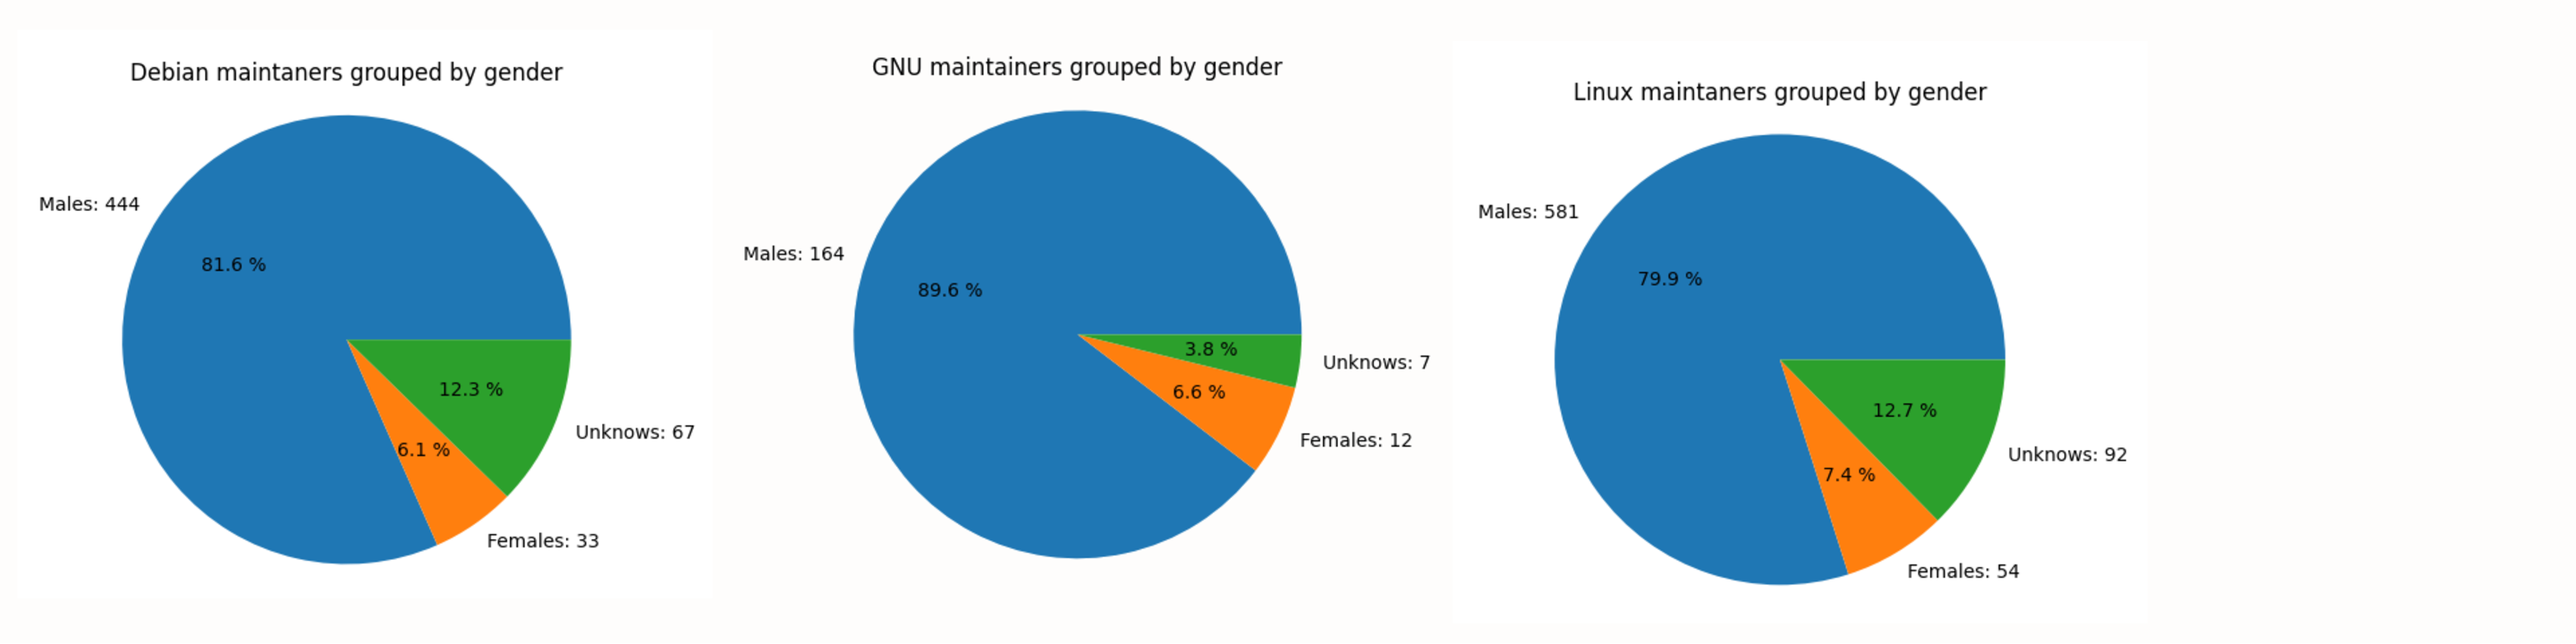
\includegraphics[width=0.6\textwidth]{images/debian-gnu-linux.pdf}     
  \caption[Caption for LOF]{Males (blue), Females (orange) and Unknows (green) in Debian, GNU and Linux}
\end{figure}

The inter dataset was created merging several open datasets downloaded
from official statistics sites from different nations: Austria,
Australia, Belgium, Canada, Germany, Denmark, Spain, Finland, Ireland,
Iceland, Mexico, New Zealand, Portugal, Slovenia, United States of
America, Uruguay and France. That's a good representation of the
Western World and the Free Software world is populating this world's
area\cite{gonzalez2008geographic}.

%% CITATION
%% ~\cite{gonzalez2008geographic}.

Linux divides the developers in 537 males (73.9\%), 98 females
(13.5\%) and 92 unknows (12.7\%). The number of unknows is due to
different reasons, but it's so common in Linux that the developer is a
company and not a name of a person.

GNU divides the developers in 164 males (89.6\%), 12 females (6.6\%)
and 7 unknows (3.8\%)

The GNU people has a number lowest in females, they are the founder of
the Free Software philosophy, the Debian principles and the Open
Source philosophy was invented later influenced by GNU with very
similar practical decisions (for example: deciding licenses for the
software). Richard Stallman returned to be president recently
apologizing by his personal behaviour with the
females.\footnote{https://www.fsf.org/news/rms-addresses-the-free-software-community}

Debian is a distribution, the project who makes the CD/DVD and the
software ready to be downloaded from Internet with the
dependencies. There are many distributions, such as, Ubuntu or RedHat
so it is not representative, but it's interesting to understand that
the numbers are similar in Debian dividing the developers in 408 males
(75\%), 69 females (12.7\%) and 67 unknows (12.3\%).

%% 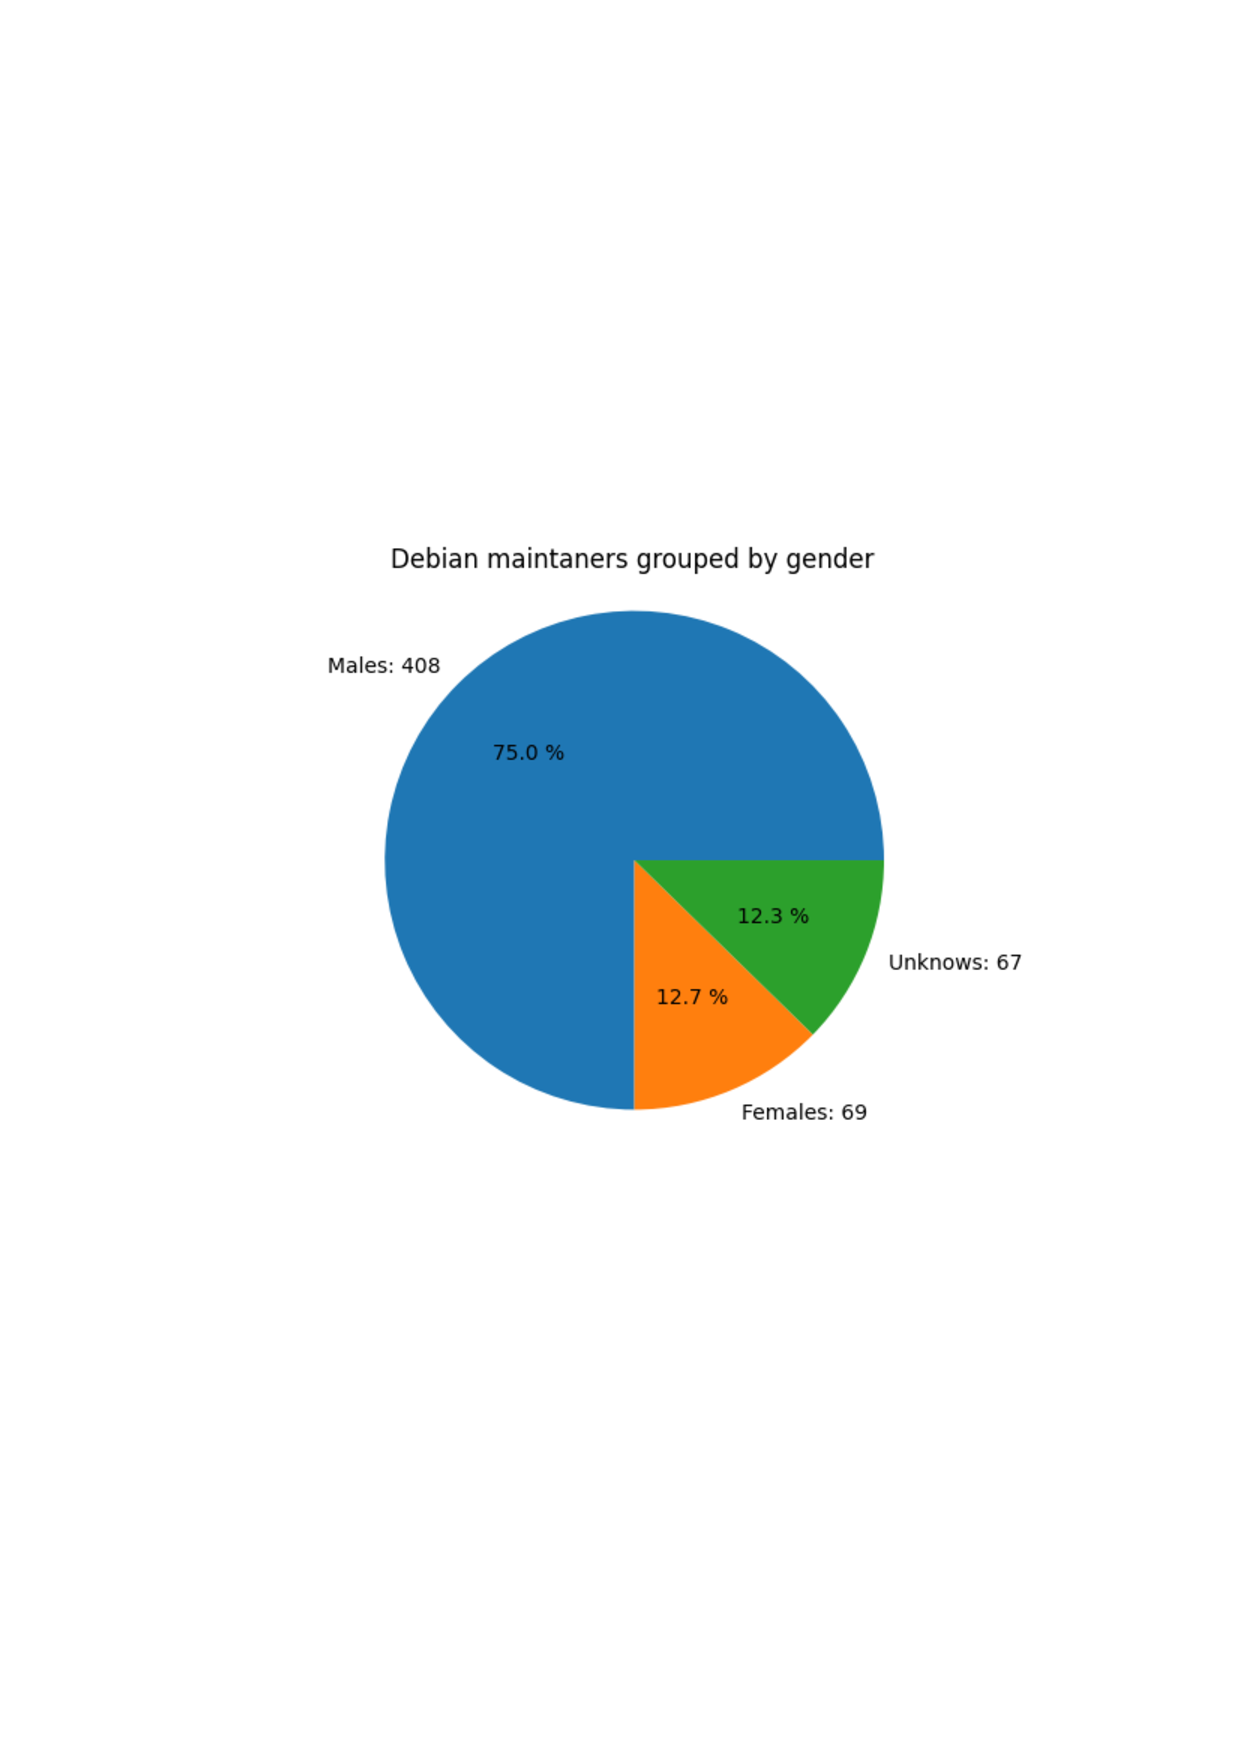
\includegraphics[width=0.9\textwidth]{images/debian-maintainers.gender.pdf}

\section{Conclusions}
\label{sec:conclusions}

This paper is explaining the application about Damegender, the
motivations (reproducible research, fix gender gap to reach an
objective of United Nations, fields of application: lingüistic, social
sciences, software engineering, natural language processing, ...)

A good solution is to build an international, universal and free
dataset about names, gender and frequency with the right design with
the current state of the job, attending to the diversity (LGTB
options, cultural minorities, ...).

The current state of work is the longest Open Dataset about names,
gender and frequency with more than 20 countries representing the
Western World, being a solution with low number of unknows in the real
world.

%% These data reveals that the situation has been improved with respect
%% the long time. In \cite{10.1007/978-3-319-39225-7_13} speaks about a
%% female participation of around 2 {\%} to 5 {\%}.

%% \section*{Acknowledgments}

%% We would like to thank: Statistical institutions by release Open
%% Datasets about names, gender and frequency. Daniel Izquierdo and Laura
%% Arjona for starting this research field at URJC all those working with
%% Jesus González Barahona and Gregorio Robles.

\bibliographystyle{alpha} 
\bibliography{uc3m}

\end{document}


